\documentclass{beamer}
\usetheme{CambridgeUS}
\usecolortheme{beaver}
\usepackage{amsmath,amssymb,enumerate,amsthm}
\usepackage{bm}

\newcommand{\profile}{\bm{v}}%(complete) profile
\newcommand{\pprofile}{{\bm{p}}}%partial profile
\newcommand{\w}{\bm{w}}
\newcommand{\W}{\mathcal{W}}
\newcommand{\Co}{\mathcal{C}}
\newcommand{\pw}{W}%our knowledge about the weights
\newcommand{\strat}[1]{\emph{#1}}
\newcommand{\ppref}{\succ^\text{p}}%partial pref
\newcommand{\pprefeq}{\succeq^\text{p}}%partial pref
\newcommand{\pref}{\succ}% pref
\DeclareMathOperator{\Regret}{Regret}
\DeclareMathOperator{\SCORE}{Score}
\DeclareMathOperator{\PMR}{PMR}
\DeclareMathOperator{\MR}{MR}
\DeclareMathOperator{\MMR}{MMR}

\makeatletter
\defbeamertemplate*{title page}{mydefault}[1][]
{
	\vbox{}
	\vfill
	\begin{centering}

%{\usebeamercolor[fg]{titlegraphic}\inserttitlegraphic\par}
		\begin{beamercolorbox}{titlegraphic}
				\usebeamerfont{titlegraphic}\inserttitlegraphic
		\end{beamercolorbox}%
			\vskip1em\par	
		\begin{beamercolorbox}[rounded=true, center, shadow=true, sep=8pt,#1]{title}
			\usebeamerfont{title}\inserttitle\par%
			\ifx\insertsubtitle\@empty%
			\else%
			\vskip0.5em%
			{\usebeamerfont{subtitle}\usebeamercolor[fg]{subtitle}\insertsubtitle\par}%
			\fi%     
		\end{beamercolorbox}%
		\vskip1em\par
		\begin{beamercolorbox}[sep=8pt,center,#1]{author}
			\usebeamerfont{author}\insertauthor
		\end{beamercolorbox}
		\begin{beamercolorbox}[sep=8pt,center,#1]{institute}
			\usebeamerfont{institute}\insertinstitute
		\end{beamercolorbox}
		\begin{beamercolorbox}[sep=8pt,center,#1]{date}
			\usebeamerfont{date}\insertdate
		\end{beamercolorbox}\vskip0.5em
		\begin{beamercolorbox}[sep=8pt,center,#1]{logo}
			\usebeamerfont{titlegraphic}\insertlogo
		\end{beamercolorbox}%
	\end{centering}
	\vfill
}
\setbeamertemplate{title page}[mydefault]
\makeatother



\titlegraphic{
\includegraphics[width=50mm]{logo_dauphine} \hspace*{5.5cm} 
\includegraphics[width=7mm]{cnrs}}
\title[Elicitation of Incomplete Preferences]{Simultaneous Elicitation of Committee and \\ Voters' Preferences}
\institute[]{$^1$ LAMSADE, Université Paris-Dauphine, Paris, France \\ $^2$ LIP6, Sorbonne Universit\'e, Paris, France}
\author[B. Napolitano, O. Cailloux, P. Viappiani]{B. Napolitano$^1$, O. Cailloux$^1$ and P. Viappiani$^2$}
%
%\title[Elicitation and Explanation in Social Choice]{Elicitation and Explanation in Social Choice Theory}
%%\subtitle{Proposal: ``Elicitation and Explanation for Voting Rules''}
%\author[Beatrice Napolitano]{\textbf{Beatrice Napolitano} \\
%	Supervisors: Remzi Sanver, Olivier Cailloux}
\date[28 June 2019]{{\small International Summer School on Preferences, Decisions and Games} \\ 28 June 2019 \\ 
\includegraphics[width=35mm]{LOGO_LAMSADE} }

\usepackage{tikz}
\usepackage{amsmath}
\usepackage{graphicx}

\definecolor{darkred}{rgb}{0.8,0,0}

\begin{document}

\beamertemplatenavigationsymbolsempty

\begin{frame}[plain]
\maketitle
\end{frame}

\addtocounter{framenumber}{-1}


\section{Setting}
\subsection{Scenario}

\begin{frame}
\frametitle{Scenario}
%\framesubtitle{Robust Winner Determination}
%	\textbf{Setting}: Two kind of players
\textbf{Setting}: Incompletely specified profile and positional scoring rule
\begin{figure}
	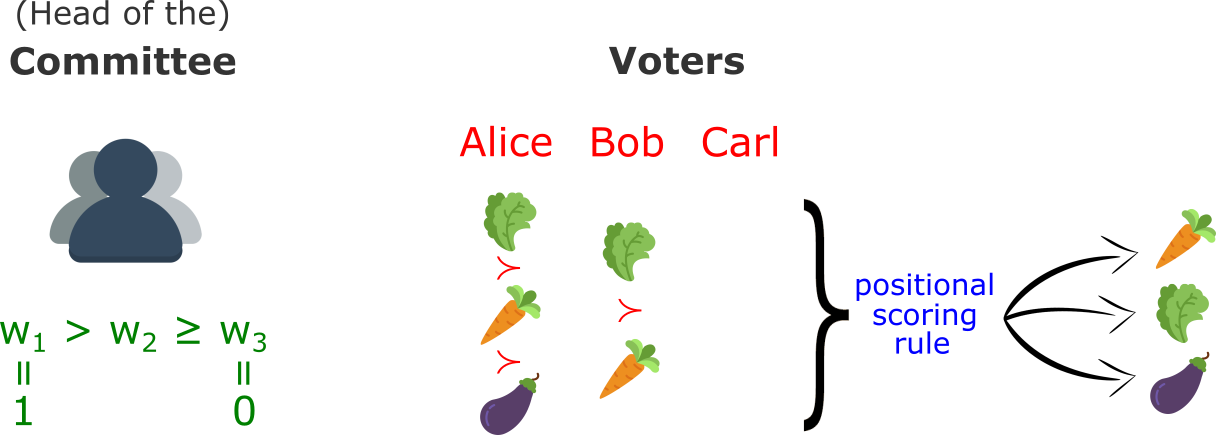
\includegraphics[scale=0.35]{setting.png}
	%		\caption{.}
	%		\label{fig:b1}
\end{figure}
\textbf{Goal}: Development of an incremental elicitation protocol based on minimax regret 
\end{frame}
%\addtocounter{framenumber}{-1}
%\begin{frame}
%	\frametitle{Scenario}
%	\textbf{Setting}: Incompletely specified profile and positional scoring rule
%	\begin{figure}
%		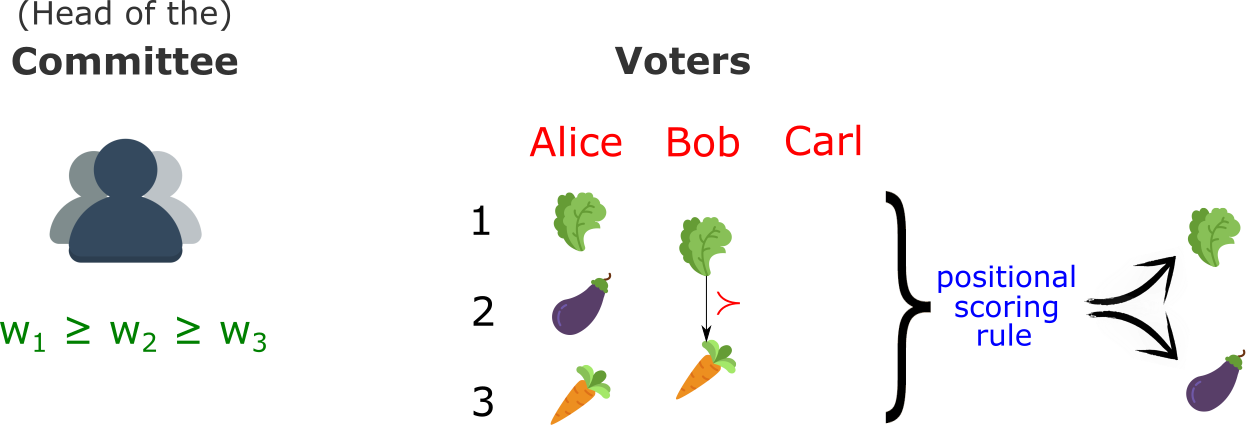
\includegraphics[scale=0.35]{set2.png}
%%		\caption{.}
%%		\label{fig:b1}
%	\end{figure}
%	\textbf{Goal}: Development of an incremental elicitation protocol based on minimax regret 
%\end{frame}

\subsection{Motivation and approach}
\begin{frame}
	\frametitle{Motivation and approach}
	\textbf{Who?}
	\begin{itemize}
		\item Imagine to be an \emph{external observer} helping with the voting procedure
	\end{itemize}
	\textbf{Why?}
	\begin{itemize}
		\item Voters: difficult or costly to order \emph{all} alternatives
		\item Committee: difficult to \emph{specify} a voting rule precisely and abstractly
	\end{itemize}
	\textbf{How?}
	\begin{itemize}
		\item \emph{Minimax regret}: given the current knowledge, the alternatives with the lowest worst-case regret are selected as tied winners
	\end{itemize}		
\end{frame}

\subsection{Related Works}
\begin{frame}
	\frametitle{Related Works}
	\textbf{Incomplete profile}  
	\begin{itemize}
		\item and known weights: Minimax regret to produce a robust winner approximation (\textit{Lu and Boutilier 2011}, \cite{Lu2011}; \textit{Boutilier et al. 2006}, \cite{Boutilier2006})
	\end{itemize}~\\
	\textbf{Uncertain weights} 
	\begin{itemize}
		\item and complete profile: dominance relations derived to eliminate alternatives always less preferred than others (\textit{Stein et al. 1994}, \cite{Stein1994})
		\item in positional scoring rules (\textit{Viappiani 2018}, \cite{Viappiani2018})
	\end{itemize}
\end{frame}

\subsection{Framework}
\begin{frame}
	\frametitle{Framework}
	
	\begin{description}[$|N|=n, |A|=m$]
		\item[$|N|=n, |A|=m$] voters, alternatives
		\item[$\ppref_j$] partial preference order of the voter $j \in N$
		\item[$\Co_W$] set of linear  constraints given by the committee about $\w$
	\end{description}
	\medskip
	Given complete voters preferences $\profile$, a specific positional scoring rule, defined by a scoring vector $\w$, attributes a score {\color{blue} $s^{\profile, \w}$} to each alternative
\end{frame}

\begin{frame}
	\frametitle{Framework}
	\begin{block}{Assumptions}
		\begin{itemize}
			\item Voters and committee have true preferences in mind
			\item The voting rule is a Positional Scoring Rule where the scoring vector $\w=(w_1, \dots , w_m)$ is a convex sequence of weights	and $w_1=1$, $w_m=0$ 
		\end{itemize}
	\end{block}
\end{frame}

\section{Minimax Regret}
\subsection{Definition}
\begin{frame}
	\frametitle{Minimax Regret}
	\begin{description}[$\mathbf{\PMR^{\pprofile,W}(x,y)}$]
		\item[$\mathbf{\PMR^{\pprofile,W}(x,y)}$] is the maximum difference of score between $x$ and $y$ under all possible realizations of the full profile {\em and} weights
		\item[$\mathbf{\MR^{\pprofile,W}(x)}$] represents the worst case loss: the \emph{maximal regret} between a chosen alternative x and best real alternative y
	\end{description}
	\bigskip		
		\centerline{\textbf{We select the alternative which \emph{minimizes} the maximal regret}}
\end{frame}

\subsection{Pairwise Max Regret Computation}
\begin{frame}
	\frametitle{Pairwise Max Regret Computation}
	The computation of $\PMR^{\pprofile,W}(x,y)$ can be seen as a game in which an adversary can both
	\begin{itemize}
		\item \textbf{complete the partial profile}\\
		\medskip
		\begin{center}
			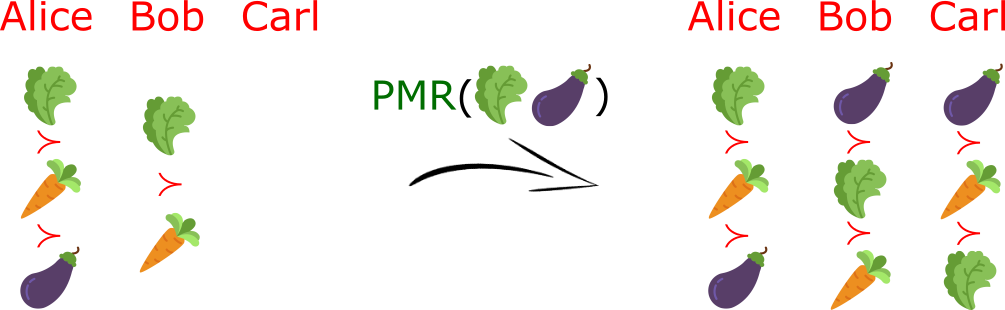
\includegraphics[scale=0.35]{completion.png}
		\end{center}
		
		\item \textbf{choose a feasible weight vector}\\
		\medskip
		\centerline{\color{red}$\mathbf{(1,0,0)}$}
	\end{itemize}
	\medskip
	in order to maximize the difference of scores
\end{frame}

\section{Elicitation}
\subsection{Question Types}
	\begin{frame}
		\frametitle{Question Types}
		\textbf{Questions to the voters}
		\begin{itemize}
			\item[] Comparison queries that ask a particular voter to compare two alternatives
			\color{blue}\[x \pref_j y \quad ?\]
		\end{itemize}
		\textbf{Questions to the committee}
		\begin{itemize}
			\item[] Queries relating the difference between the importance of consecutive ranks $r$ and $r+1$
			\color{blue} \[ w_{r} - w_{r+1} \geq \lambda (w_{r+1} - w_{r+2}) \quad ? \] 
		\end{itemize}
	\end{frame}
	
	\subsection{Elicitation strategies}
	\begin{frame}
		\frametitle{Elicitation strategies}
		\begin{itemize}
			\item \textbf{Random}: equiprobably draws a question among the set of the possible ones;
			
			\item \textbf{Extreme completions}: choses the question that reduces the most the uncertainty;
			
			\item \textbf{Pessimistic}: selects the question that leads to minimal regret in the worst case; 
			
			\item \textbf{Two phase}: it asks a predefined sequence of questions to the committee and then it only asks questions about the voters.
		\end{itemize}
		\bigskip
	\end{frame}


\addtocounter{framenumber}{-1}
\begin{frame}[plain]
	\centering \color{darkred}\LARGE Thank You!
\end{frame}




\bibliographystyle{plain}
\bibliography{biblio} 
%given a combination of axioms we want to find an outcome that doesn't satisfy them, and we would do that for several reasons:
%-querying the user, depending of her answer we might infer her preferences over the set of axioms;
%-proving that a set of axioms is not valid giving a counter-example;


%A method for automatically proving impossibility theorems in the area of ranking sets of objects has already been implemented (Geist \& Endriss, 2011). It:



\end{document}